%
% slides.tex -- slides
%
% (c) 2017 Prof Dr Andreas Müller, Hochschule Rapperswil
%
\theoremstyle{definition}
\newtheorem{wien}{Wiensches Verschiebungsgesetz}
\newtheorem{planck}{Plancksches Strahlungsgesetz}

\begin{document}

\ifthenelse{\boolean{presentation}}{
\begin{frame}
\titlepage
\end{frame}
}{}

\begin{frame}
\frametitle{Bodyko-Modell 1}
Modellannahmen:
\begin{enumerate}
\item Einfallende Strahlung
\[
E_{\text{in}}
=
\frac{\text{Solarstrahlung auf Erdquerschnitt}}{\text{verteilt über Kugeloberfläche}}
=
\frac{\pi R^2 S_0}{4\pi R^2}=\frac{S_0}{4}
\]
\item Verlust durch Albedo
\[
E_{\text{in}}
=
(1-\alpha)\frac{S_0}{4} = (1-\alpha)Q
\]
\item Stefan-Boltzmann-Gesetz
\[
\color{blue}
E_{\text{out}}(T)=\sigma T^4
\]
\end{enumerate}
Gleichgewichtsbedingung:
\[
(1-\alpha)Q=\sigma T^4
\qquad\Rightarrow\qquad
T^* = \biggl(
\frac{(1-\alpha)Q}{\sigma}
\biggr)^{\frac14}
\]
\end{frame}

\begin{frame}
\frametitle{Budyko-Modell 2}
Albedo hängt von der Temperatur ab:
\begin{center}
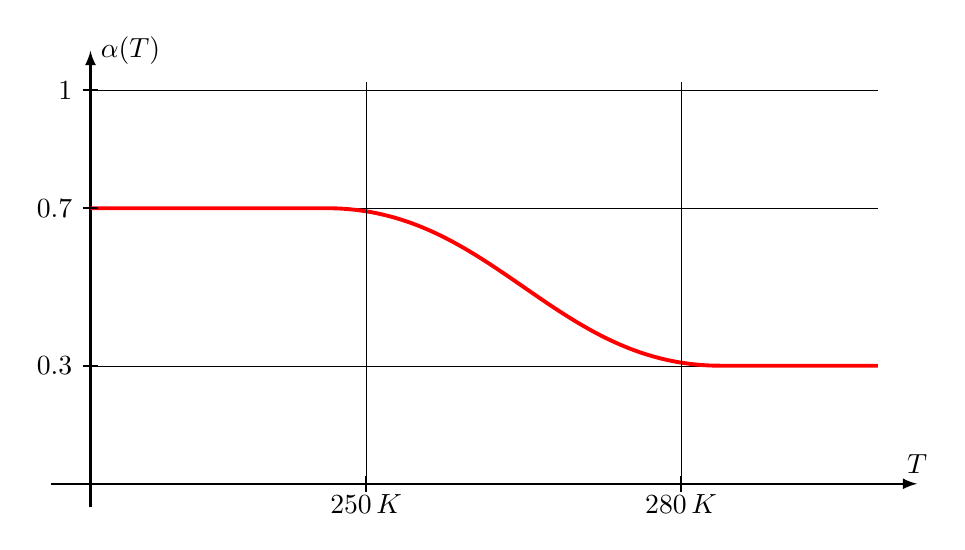
\begin{tikzpicture}[>=latex,thick]
\draw[->] (-0.5,0)--(10.5,0) coordinate[label=$T$];
\draw[->] (0,-0.3)--(0,5.5) coordinate[label={right:$\alpha(T)$}];
\draw (-0.1,5)--(0.1,5);
\node at (-0.1,5) [left] {$1$};
\node at (-0.1,{5*0.3}) [left] {$0.3$};
\node at (-0.1,{5*0.7}) [left] {$0.7$};
\draw[line width=0.1pt] (0,5)--(10,5);
\draw[line width=0.1pt] (0,{5*0.7})--(10,{5*0.7});
\draw[line width=0.1pt] (0,{5*0.3})--(10,{5*0.3});
\draw[color=red,line width=1.4pt] (0,{5*0.7})--(3,{5*0.7})
	to[out=0,in=180] (8,{5*0.3})--(10,{5*0.3});
\draw (-0.1,{5*0.3})--(0.1,{5*0.3});
\draw (-0.1,{5*0.7})--(0.1,{5*0.7});
\draw (3.5,-0.1)--(3.5,0.1);
\draw (7.5,-0.1)--(7.5,0.1);
\node at (3.5,0) [below] {$250\,\text{K}$};
\node at (7.5,0) [below] {$280\,\text{K}$};
\draw[line width=0.1] (3.5,0)--(3.5,5.1);
\draw[line width=0.1] (7.5,0)--(7.5,5.1);
\end{tikzpicture}
\end{center}
\end{frame}

\begin{frame}
\frametitle{Gleichgewichtslösungen}
\begin{center}
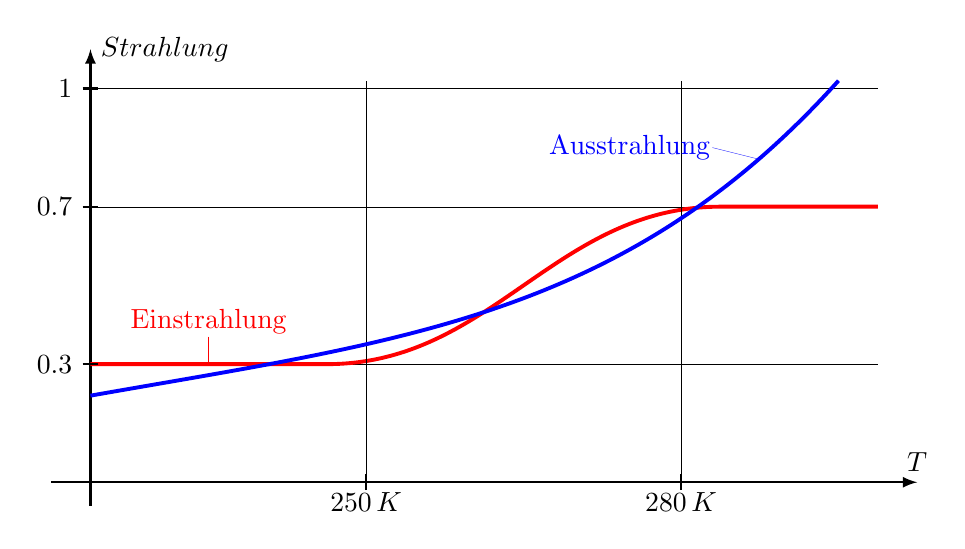
\begin{tikzpicture}[>=latex,thick]
\draw[->] (-0.5,0)--(10.5,0) coordinate[label=$T$];
\draw[->] (0,-0.3)--(0,5.5) coordinate[label={right:$\text{Strahlung}$}];
\draw (-0.1,5)--(0.1,5);
\node at (-0.1,5) [left] {$1$};
\node at (-0.1,{5*0.3}) [left] {$0.3$};
\node at (-0.1,{5*0.7}) [left] {$0.7$};
\draw[line width=0.1pt] (0,5)--(10,5);
\draw[line width=0.1pt] (0,{5*0.7})--(10,{5*0.7});
\draw[line width=0.1pt] (0,{5*0.3})--(10,{5*0.3});
\draw[color=red,line width=1.4pt] (0,{5*0.3})--(3,{5*0.3})
	to[out=0,in=180] (8,{5*0.7})--(10,{5*0.7});
\draw (-0.1,{5*0.3})--(0.1,{5*0.3});
\draw (-0.1,{5*0.7})--(0.1,{5*0.7});
\draw (3.5,-0.1)--(3.5,0.1);
\draw (7.5,-0.1)--(7.5,0.1);
\node at (3.5,0) [below] {$250\,\text{K}$};
\node at (7.5,0) [below] {$280\,\text{K}$};
\draw[line width=0.1] (3.5,0)--(3.5,5.1);
\draw[line width=0.1] (7.5,0)--(7.5,5.1);
\draw[color=blue,line width=1.4pt] (0,{5*0.22}) to[out=10,in=-132] (9.5,5.1);
\node[color=red] at (1.5,{5*0.35}) [above] {Einstrahlung};
\draw[color=red,line width=0.1pt] (1.5,{5*0.37})--(1.5,{5*0.3});
\node[color=blue] at (8,{5*0.85}) [left] {Ausstrahlung};
\draw[color=blue,line width=0.1pt] (7.9,{5*0.85})--(8.5,{5*0.82});
\end{tikzpicture}
\end{center}
\vspace{-15pt}
\uncover<2->{$\Rightarrow$ 3 Gleichgewichtslösungen}%
\uncover<3->{, Temperatursprünge möglich}
\end{frame}

\begin{frame}
\frametitle{Strahlungsspektrum}
Es fehlt: spektrale Abhängigkeit der Strahlung
\uncover<2->{
\begin{planck}
Strahler, dessen Spektrum nur von der Temperatur abhängt:
\[
E(\lambda,T)
=
\frac{2\pi hc^2}{\lambda^5} \frac{1}{e^{\frac{hc}{\lambda kT}}-1}
\uncover<3->{
\qquad\Rightarrow\qquad
E(T)
=\int_0^\infty \frac{2\pi hc^2}{\lambda^5} \frac{1}{e^{\frac{hc}{\lambda kT}}-1}
\,d\lambda
}
\]
\end{planck}
}
\uncover<4->{
Daraus kann man das Stefan-Boltzmann-Gesetz $E(T)=\sigma T^4$ ableiten
}
\uncover<5->{
\begin{wien}
Strahlungsmaximum ist proportional zu $1/T$:
\[
\lambda_{\text{max}}
=
\frac{b}{T}
\qquad\text{mit}\qquad
b=2.897\cdot10^{-3}\,\text{m}\cdot\text{K}
\]
\end{wien}
}
\end{frame}

\begin{frame}
\frametitle{Sonnenspektrum}
\begin{columns}
\begin{column}{0.61\hsize}
\vspace{-15pt}
\begin{center}
\begin{tikzpicture}[>=latex,thick]
\node at (0,0) {
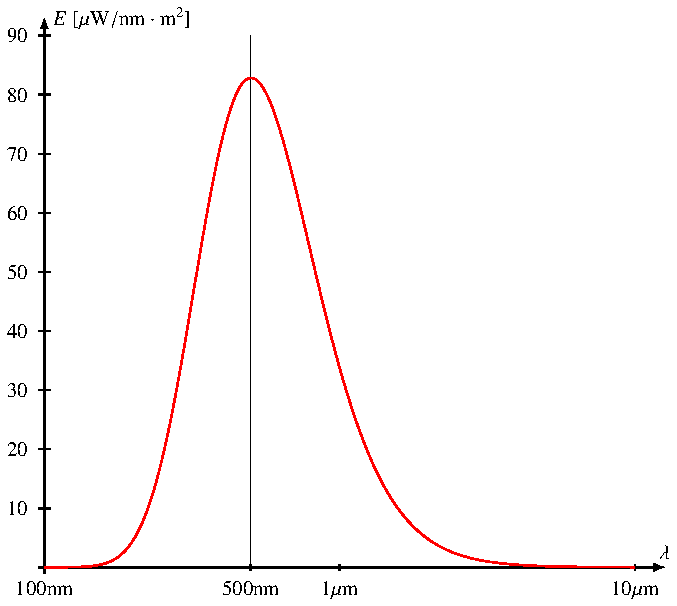
\includegraphics[width=\hsize]{../../skript/chapters/1/planck.pdf}
};
\uncover<2->{
\node at (-0.98,-1) {

\includegraphics[width=0.1\hsize]{spektrum.png}
};
}
\end{tikzpicture}
\end{center}
\end{column}
\begin{column}{0.40\hsize}
\begin{itemize}[<+->]
\item Maximum bei 500nm (grün)
\item Sichtbare Strahlung zwischen 390nm und 700nm
\item Solarspektrum wird als ``weiss'' empfunden
\item Lichtquellen mit höherer Temperatur erscheinen bläulich,
Quellen mit tieferer Temperatur dagegen rötlich
\end{itemize}
\end{column}
\end{columns}
\end{frame}

\begin{frame}
\begin{center}
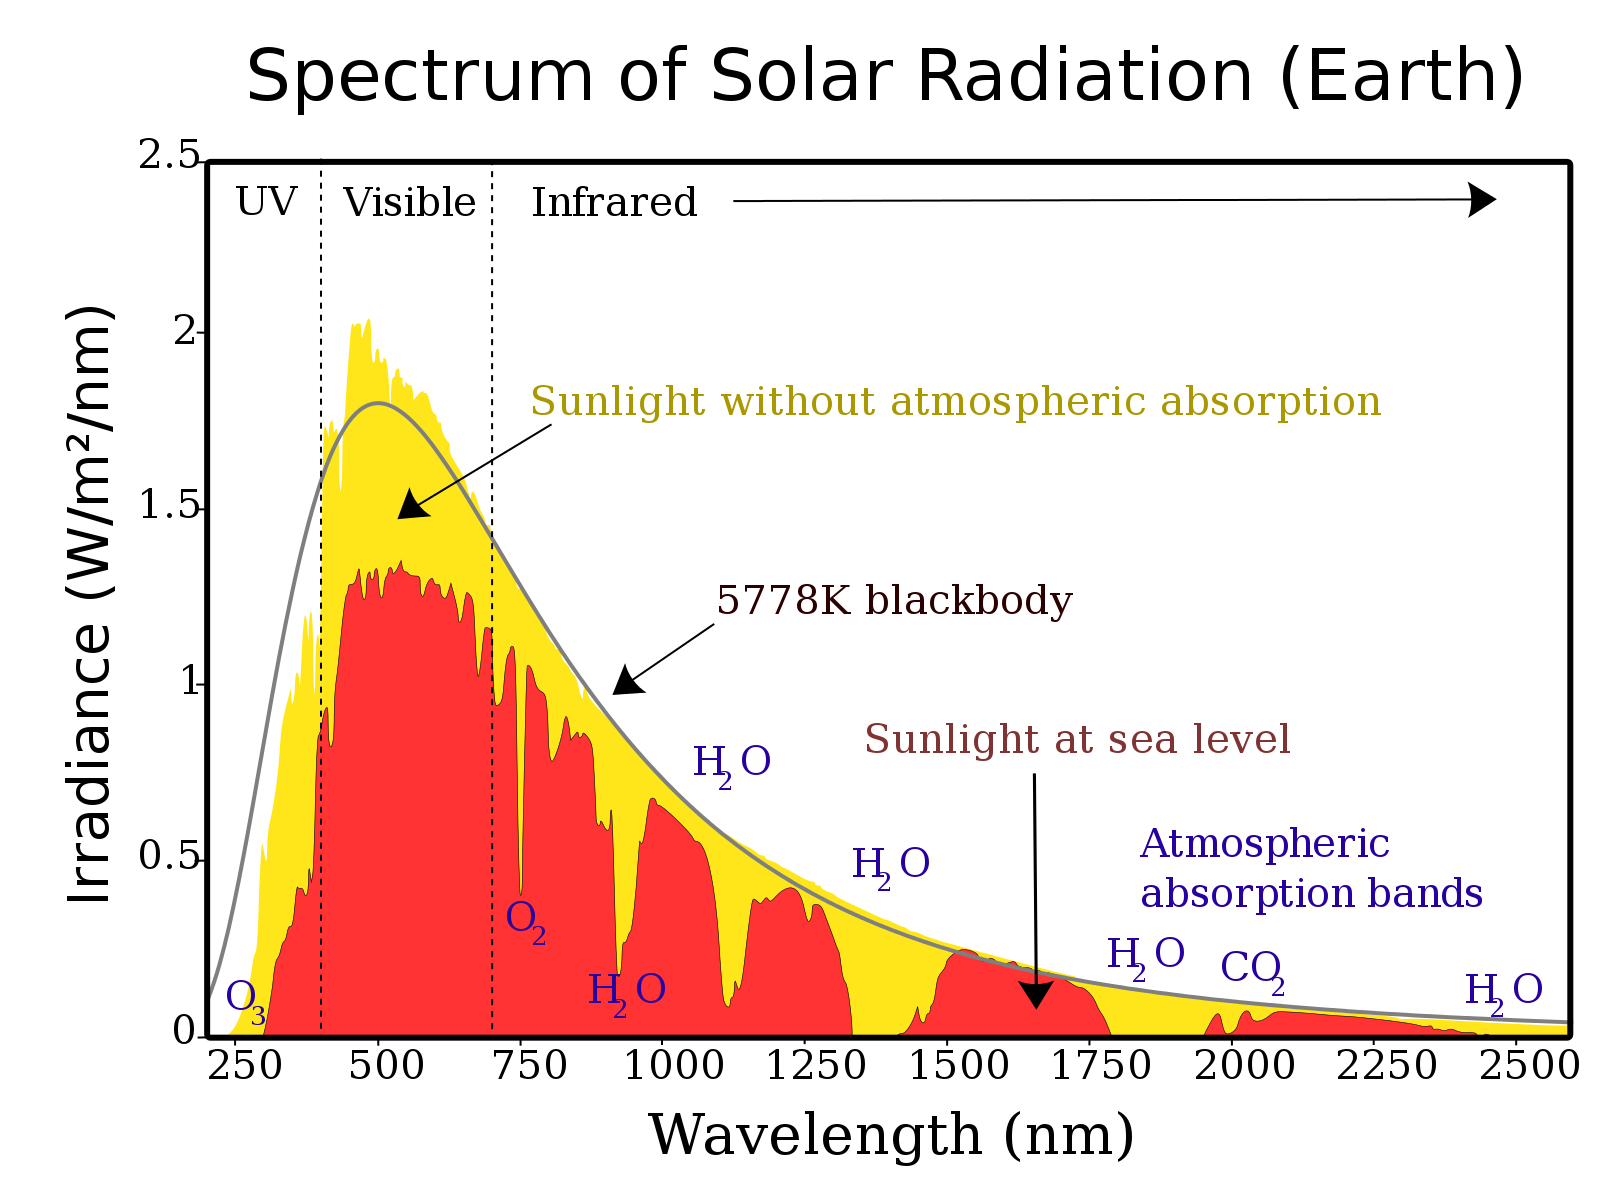
\includegraphics[width=0.85\hsize]{../../skript/chapters/1/Solar_spectrum_en.png}
\end{center}
\end{frame}

\begin{frame}
\frametitle{Vergleich}
In einer logarithmischen Skala derart, dass $E(T)$ direkt der Fläche unter
der Kurve entspricht, werden $\color{red}E(T_{\text{Sonne}})$ und
$\color{blue}E(T_{\text{Erde}})$
vergleichbar
\begin{center}
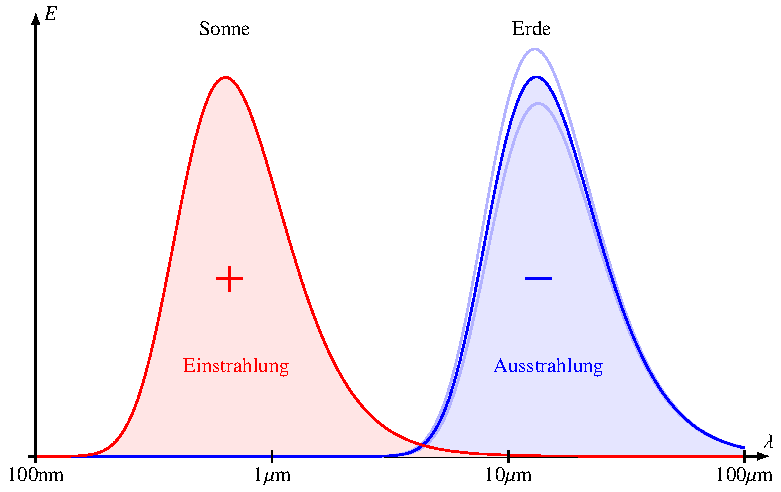
\includegraphics[width=0.7\hsize]{../../skript/chapters/1/vergleich.pdf}
\end{center}
\end{frame}


\end{document}
